\documentclass{beamer}

\mode<article> % only for the article version
{
	\usepackage{fullpage}
	\usepackage{hyperref}
}

\mode<presentation>
{
	\usetheme{boxes}
	\usetheme{JuanLesPins}
}

\usepackage{astron}
\usepackage{gastex}
\usepackage{multirow}

\usepackage{pgf,pgfarrows,pgfnodes,pgfautomata,pgfheaps,pgfshade}
\setbeamercovered{dynamic}

%Include Macro commands
%To comment out some parts for submission
\newcommand{\commM}[1]{}
\newcommand{\commE}[1]{#1}

%Frame box for formulas with minipage
\newsavebox{\ffrbox}
\newenvironment{fframe}[2] {\begin{center} \begin{lrbox}{\ffrbox} \begin{minipage}{#1\linewidth} \vspace{#2cm}}{ \end{minipage} \end{lrbox} \fbox{\usebox{\ffrbox}} \end{center}}

%Eigenvalue eigenvector
\newcommand{\vx}[1]{\overrightarrow{x_{#1}}}
\newcommand{\vxe}{\overrightarrow{x^{*}}}
\newcommand{\vxi}[1]{\overrightarrow{x\left(#1\right)}}
\newcommand{\xij}[1]{x\left(#1\right)_{j}}
\newcommand{\vxl}{\vx{\lambda}}
\newcommand{\vxli}[1]{\vx{\lambda_{#1}}}
\newcommand{\vp}{\overrightarrow{p}}

%Matric & vector norms
\newcommand{\nvec}[1]{\lVert #1 \rVert_{v} }
\newcommand{\nmat}[1]{\lVert #1 \rVert_{m} }
\newcommand{\nvece}[1]{\nvec{ #1 }^{2} }
\newcommand{\nvecinf}[1]{\nvec{ #1 }^{\infty} }
\newcommand{\nvecinfal}[1]{\nvec{ #1 }^{{\color[rgb]{0,0,1}\infty}} }
\newcommand{\nmatinf}[1]{\nmat{ #1 }^{\infty} }
\newcommand{\jinlN}[3]{#1 \in #2,..,#3} %\overline{}
\newcommand{\vInd}{\overrightarrow{i_{Ind}}}

%Complexity
\newcommand{\Oc}[1]{\mathcal{O}\left( #1 \right)} %Big o - i.e. time complexity

%Uniformization
\newcommand{\ur}{q} %uniformization rate

%CTMC & DTMC matrices
\newcommand{\mB}{\mP_{B}} %A DTMC where all bad states, i.e. not Phi and not Psi and Psi belonging to some BSCC are made absorbing
\newcommand{\mP}{\mathcal{P}} %A stochastic matrix
\newcommand{\mU}{\mP_{unif}} %Uniformized CTMC
\newcommand{\mT}{\mathcal{T}} %An irreducible submatrix of a stochastic matrix.
\newcommand{\DTMC}{\left( S,\: \mP \right)}
\newcommand{\mQ}{\mathcal{Q}} %Generator matrix
\newcommand{\mR}{\mathcal{R}} %Rate matrix
\newcommand{\CTMC}{\left( S,\: \mQ \right)}
\newcommand{\mA}{\mathcal{A}}
\newcommand{\mQnpvp}{\mQ\left[\npvp \right]}
\newcommand{\mQBnpvp}{\mQ^{B}\left[\npvp \right]}

%CTMC and transient analysis
\newcommand{\pipOti}{\pi^{*} \left(0, t \right )_{i}} %The i'th component of \vpipOt
\newcommand{\vpipOt}{\overrightarrow{\pi^{*} \left(0, t \right )}} % Transient probability, precise
\newcommand{\pipOtj}{\pi^{*} \left(0, t \right )_{j}} % The j'th component of the transient-probability vector, precise
\newcommand{\vpiOt}{\overrightarrow{\pi \left(0, t \right )}} % Transient probability, computed
\newcommand{\piOtj}{\pi \left(0, t \right )_{j}} % The j'th component of the transient-probability vector, computed


\newcommand{\pOi}{p\left( 0 \right)_{i}} % The i'th component of \vpO
\newcommand{\vpO}{\overrightarrow{p \left( 0 \right)} } % Initial distribution for a CTMC
\newcommand{\vpOi}{\overrightarrow{p(0,i)}} %The i'th iteration for uniformized DTMC, with initial distribution \vpiO
\newcommand{\pOij}{p(0,i)_{j}} %The j'th component of \vpOi
\newcommand{\vpOK}{\overrightarrow{p(0,K)}} %The K'th iteration for uniformized DTMC, with initial distribution \vpiO
\newcommand{\pOKj}{p(0,K)_{j}} %The j'th component of \vpOK
\newcommand{\vpOiM}{\overrightarrow{p(0,i+M)}} %The (i+M)'th iteration for uniformized DTMC, with initial distribution \vpiO
\newcommand{\vppO}{\overrightarrow{p^{*}(0)}} %The steady state for transient analysis, starting in state \vpiO
\newcommand{\ppOj}{p^{*}(0)_{j}} %The j'th component of \vppO
\newcommand{\ppOi}{p^{*}(0)_{i}} %The i'th component of \vppO

%CSL model checking
\newcommand{\vis}{\overrightarrow{1_{s} }} %The initial distribution for state s
\newcommand{\vpist}{\overrightarrow{\pi \left( s,t \right) }}
\newcommand{\vpit}{\overrightarrow{\pi \left( t \right) }} %The resulting probability vector for backward computations
\newcommand{\vpsi}{\overrightarrow{p(s,i)}} %An i'th iteration vector for forward computation 
\newcommand{\vpsj}[1]{\overrightarrow{p(s,#1)}} %An j'th iteration vector for forward computation 
\newcommand{\vpsim}{\overrightarrow{p(s,i{+}M)}}  %An (i+m)'th iteration vector for forward computation
\newcommand{\vpOim}{\overrightarrow{p(0,i{+}M)}}  %An (i+m)'th iteration vector for forward computation
\newcommand{\vpsK}{\overrightarrow{p(s,K)}} %A K'th iteration vector for forward computation 
\newcommand{\vpsKI}{\overrightarrow{p(s,K{+}1)}} %A K+1'th iteration vector for forward computation 
\newcommand{\vpi}{\overrightarrow{p(i)}} %An i'th iteration vector for backward computation
\newcommand{\vpK}{\overrightarrow{p(K)}} %An K'th iteration vector for backward computation
\newcommand{\vpKI}{\overrightarrow{p(K{+}1)}} %An K+1'th iteration vector for backward computation
\newcommand{\vpiM}{\overrightarrow{p(i{+}M)}} %An (i+m)'th iteration vector for backward computation
\newcommand{\vpipt}{\overrightarrow{\pi^{*} \left( t \right)}} % A precise solution of equation for backward computations
\newcommand{\vpipst}{\overrightarrow{\pi^{*} \left(s, t \right)}}  % A precise solution of equation for forward computations
\newcommand{\vpps}{\overrightarrow{p^{*}(s)}} % The precise steady-state vector for forward computation
\newcommand{\vpp}{\overrightarrow{p^{*}}} % The precise steady-state vector for backward computation
\newcommand{\vipsi}{\overrightarrow{i_{\Psi}}}
\newcommand{\vibad}{\overrightarrow{i_{\BPsi \cup \SNPhi}}}
\newcommand{\vbpi}{\overrightarrow{p^{B}\left( i \right)}}
\newcommand{\vbpK}{\overrightarrow{p^{B}\left( K \right)}}
\newcommand{\bpij}{p^{B}\left( i \right)_{j}}

\newcommand{\ipsij}{i_{\Psi,j}}  %The j'th component of \vipsi
\newcommand{\pitj}{\pi \left( t \right)_{j}}
\newcommand{\pits}{\pi \left( t \right)_{s}}
\newcommand{\piptj}{\pi^{*} \left( t \right)_{j}}
\newcommand{\pipts}{\pi^{*} \left( t \right)_{s}}
\newcommand{\pistj}{\pi \left(s, t \right)_{j}}
\newcommand{\pipstj}{\pi^{*} \left(s, t \right)_{j}}
\newcommand{\pij}{p(i)_{j}} % The j'th component of the i'th iterate for backward computation
\newcommand{\pilj}{p(i+1)_{j}} % The j'th component of the i+1'th iterate for backward computation
\newcommand{\pKj}{p(K)_{j}} % The j'th component of the K'th iterate for backward computation
\newcommand{\ppj}{p^{*}_{j}} % The j'th component of the precise steady-state vector for backward computation
\newcommand{\psij}{p(s,i)_{j}} % The j'th component of the i'th iterate for forward computation starting from state s
\newcommand{\psji}[2]{p(s,#1)_{#2}} % The i'th component of the j'th iterate for forward computation starting from state s
\newcommand{\pjik}{p(j,i)_{k}} % The k'th component of the i'th iterate for forward computation, starting from state j
\newcommand{\psiNl}{p(s,i)_{N{-}1}} % The N-1'th component of the i'th iterate for forward computation
\newcommand{\psiN}{p(s,i)_{N}} % The N'th component of the i'th iterate for forward computation
\newcommand{\psKNI}{p(s,K)_{N{-}1}} % The N-1'th component of the K'th iterate for forward computation
\newcommand{\psKINI}{p(s,K+1)_{N{-}1}} % The N-1'th component of the K+1'th iterate for forward computation
\newcommand{\psKIN}{p(s,K{+}1)_{N}} % The N'th component of the K+1'th iterate for forward computation
\newcommand{\psKN}{p(s,K)_{N}} % The N'th component of the K'th iterate for forward computation
\newcommand{\psKj}{p(s,K)_{j}} % The j'th component of the K'th iterate for forward computation
\newcommand{\psKZj}{p(s,K{+}Z)_{j}} % The j'th component of the K+Z'th iterate for forward computation

\newcommand{\psKIj}{p(s,K{+}1)_{j}} % The j'th component of the K+1'th iterate for forward computation
\newcommand{\ppsj}{p^{*}(s)_{j}} % The j'th component of the precise steady-state vector for forward computation
\newcommand{\ppsNl}{p^{*}(s)_{N{-}1}} % The N-1'th component of the precise steady-state vector for forward computation
\newcommand{\ppsN}{p^{*}(s)_{N}} % The N'th component of the precise steady-state vector for forward computation

%For the stopping criteria
\newcommand{\psjk}[1]{p\left(s,#1\right)_{k}}
\newcommand{\tmaxk}{t_{k}^{max}}  %the max probability to go from a transient state to and absorbing state k in one step

%Poisson 
\newcommand{\pnd}{e^{-\ur t}\frac{\left( \ur t \right)^{i}}{i!}}
\newcommand{\gpqt}[1]{\gamma_{#1}(t)}
\newcommand{\giqt}{\gpqt{i}}
\newcommand{\gjqt}{\gpqt{j}}

%Fox-Glynn
\newcommand{\ltp}{\mathcal{L}_{\epsilon}} %Left truncation point
\newcommand{\rtp}{\mathcal{R}_{\epsilon}} %Right truncation point
\newcommand{\wi}{w_{i}(t)} %The i'th weight

%Misc
\newcommand{\ToDo}[1]{ 
                                          \begin{center} 
                                          *************************** ToDo ***************************\\
                                          \emph{#1}\\
                                          ************************************************************
                                          \end{center} 
                                        }
\newcommand{\eqnapp}[1]{
                                            \renewcommand{\theequation}{#1.\arabic{equation}}
                                            % redefine the command that creates the equation no.
                                            \setcounter{equation}{0}  % reset counter 
                                          }

%Good and Bad states
	%Sets of states
	\newcommand{\Ind}{Ind} %A set of indexes
	\newcommand{\Gl}{\mathcal{G}} %Goal states
	\newcommand{\Al}{\mathcal{A}} %Allowed states
	\newcommand{\Il}{\mathcal{I}} %Illegal states those which are no \Al and not \Gl
	\newcommand{\Bag}{B_{ \Al, \Gl }} %The bad states to make absorbing
	\newcommand{\vigl}{\overrightarrow{1_{\Gl}}}
	\newcommand{\viind}{\overrightarrow{1_{\Ind}}}
	\newcommand{\AlMBagGl}{\Al \setminus \left( \Gl \cup \Bag \right)}

	%Matrices
	\newcommand{\mQnavg}{\mQ\left[ \Il \cup \Gl \right]}

	%Probabilistic Time reachability
	\newcommand{\PZsf}[3]{\mathrm{P}_{#1}(#2, \:#3)}
	\newcommand{\ppUp}[4]{#1 \: \mathrm{U}^{[#2,#3]} \: #4}
	\newcommand{\PZsaUg}[4]{\PZsf{#1}{#2}{\ppUp{\Al}{#3}{#4}{\Gl}}}
	
	\newcommand{\PZaUg}[3]{\PZf{#1}{\ppUp{\Al}{#2}{#3}{\Gl}}}

	\newcommand{\Psf}[2]{\mbox{\it Prob}(#1, \: #2 )}
	\newcommand{\Pf}[1]{\mathrm{P}( #1 )}
	\newcommand{\PsaUg}[3]{\Psf{#1}{\ppUp{\Al}{#2}{#3}{\Gl}}}
	\newcommand{\PsSUg}[3]{\Psf{#1}{\ppUp{S}{#2}{#3}{\Gl}}}
	
	%Vectors
	\newcommand{\vibadag}{\overrightarrow {i_{\Bag \cup \Il}}}

%PRCTL
\newcommand{\Y}[2]{{\cal Y}^{#1}_{#2}}
\newcommand{\Prob}[3]{{\cal P}_{#1 #2}(#3)}

%CSL
	%Steady-state operator
	 \newcommand{\SpsP}[3]{\mathrm{S}_{\trianglelefteq #1}(#2,\: #3)}
	 
	 %Next operator
	 \newcommand{\Xp}[3]{\mathrm{X}^{[#1,\:#2]} \: #3}
	 
	%Until operator
	\newcommand{\ttUp}[2]{\ppUp{tt}{#1}{#2}{\Psi}}  %The time bounded true Until Psi formula
	\newcommand{\pUp}[2]{\ppUp{\Phi}{#1}{#2}{\Psi}}  %The time bounded Phi Until Psi formula
	
	%Bounded probability and until operator with some initial state
	\newcommand{\PZf}[2]{\mathrm{P}_{#1}(#2)}
	\newcommand{\PZspUp}[4]{\PZsf{#1}{#2}{\pUp{#3}{#4}}}
	\newcommand{\PZsttUp}[4]{\PZsf{#1}{#2}{\ttUp{#3}{#4}}}
	\newcommand{\PZpUp}[3]{\PZf{#1}{\pUp{#2}{#3}}}

	%Probability for state formula with some initial state
	\newcommand{\PspUp}[3]{\Psf{#1}{\pUp{#2}{#3}}}
	\newcommand{\PsttUp}[3]{\Psf{#1}{\ttUp{#2}{#3}}}
	
	%Some bad states, we make absorbing
	\newcommand{\BPsi}{\mathrm{B}_{\Psi}}

%CSRL
	%Until reward operator
	\newcommand{\ppUrp}[6]{#1 \: \mathrm{U}^{{\tiny [#2,#3]}}_{{\tiny [#4,#5]}} \: #6}
	\newcommand{\pUrp}[4]{\ppUrp{\Phi}{#1}{#2}{#3}{#4}{\Psi}}  %The time bounded Phi Until Psi formula

	\newcommand{\npvp}{\lnot \Phi \vee \Psi}
	\newcommand{\Sat}[1]{Sat \left(#1 \right)} % The set of states satisfying \Psi
	\newcommand{\SPsi}{\Sat{\Psi}} % The set of states satisfying \Psi
	\newcommand{\SPhi}{\Sat{\Phi}} % The set of states satisfying \Psi
	\newcommand{\SNPhi}{\Sat{\lnot \Phi}} % The set of states satisfying \not \Psi
	\newcommand{\Bpp}{B_{ \Phi, \Psi }} %The bad states to make absorbing
	\newcommand{\mQB}{\mQ^{B}} %The \mQ[\npvp] matrix with \Bpp states made absorbing

%Tools
	\newcommand{\prism}{\emph{Prism v2.1}}
	\newcommand{\etmcc}{\emph{ETMCC v1.4.2}}
	\newcommand{\mrmc}{\emph{MRMC v1.0}}
	\newcommand{\ultrasan}{\emph{UltraSAN v3.0}}


\title{On-the-fly steady-state detection for time-bounded reachability in CTMCs}
\author{Ivan S. Zapreev, Joost-Pieter Katoen}
\date{ University of Twente,\\
	RWTH Aachen\\
	{\tiny \today}
}

\begin{document}

\bibliographystyle{astron}

\frame{\titlepage}

\section[Outline]{}
\frame{\tableofcontents}

\section{Introduction}	

\frame{
       \frametitle{Outline}
       \tableofcontents[currentsection]
}

\frame
{
	\frametitle{DTMC \& CTMC}
	\begin{definition}
			A Discrete-time Markov Chain (\emph{DTMC}) is a tuple $\DTMC$ with $S$ as a finite set of states, $\mP \: : \: S \times S \rightarrow \left[0,\:1 \right]$, where $\mP=\left(p_{i,j}\right)$ and $\forall i \in S \: : \: \sum_{j=1}^{|S|}	p_{i,j}=1$,	as a state-transition probability matrix.
	\end{definition}
	\begin{definition}
			A Continuous-time Markov Chain (\emph{CTMC}) is a tuple $\CTMC$ with $S$ as a finite set of states, $\mQ \: : \: S \times S \rightarrow \mathcal{R}_{\geq 0}$, where $\mQ=\left(q_{i,j}\right)$ and $\forall i \in S \: : \: q_{i,i} = -\sum_{j, \: i \neq j} q_{i,j}$, as a generator matrix.
			Here $\forall i \neq j$, $q_{i,j}$ defines the rate of going from state $i$ to $j$.
	\end{definition}
}

\frame
{
	\frametitle{Stationary probabilities, DTMC \cite{Haverkort_98}}
	\begin{definition}
			The \emph{stationary} or \emph{steady-state} probability of a DTMC is a vector $\vppO$ such that:
			\begin{equation}
				\vppO = lim_{n \to \infty} \: \vpO \cdot \mP^{n}
				\label{eq:ssl_dtmc}
			\end{equation}
			where $\vpO$ is the initial distribution.
	\end{definition}
	\begin{theorem}
			An irreducible and aperiodic DTMC with positive recurrent states, has a unique limiting distribution (\ref{eq:ssl_dtmc}) which does not depend on the initial distribution $\vpO$.
	\end{theorem}
}

\frame
{
	\frametitle{Power Iterations  \cite{Stewart_94}}
	{\small
	\begin{definition}
		For a stochastic matrix $\mP$:
		\begin{equation}
			\vpOi  = \vpO \cdot \mP^i, \: \vpO \textrm{ - initial vector} \nonumber
		\end{equation}
	\end{definition}
	\begin{theorem}
		 If $\mP$ is \emph{aperiodic} and \emph{irreducible} then the Power Method is guaranteed to converge to some $\vpp$.
	\end{theorem}
	\begin{lemma}
		For a stochastic matrix $\mP$, the number of iterations $K$ needed to satisfy a tolerance criterion $\epsilon$ may be approximated by:
		\begin{equation}
			K = \dfrac{\log \epsilon}{log | \lambda_{2} |}, \: \lambda_{2} \textrm{ - subd. e.v. of }\mP \nonumber
		\end{equation}
	\end{lemma}
	}
}
	
\frame
{
	\frametitle{Convergence \cite{Stewart_94}}
	
	\begin{alertblock}{Tests for convergence}
		\begin{itemize}
			\item Absolute: $\nvecinf{\vpOi - \vpOiM} \leq \epsilon$, for some $M$.
			\item Relative: $\max_{j} \left( \frac{ | \vpsim_{j} - \vpsi_{j} |}{ | \vpsim_{j}  |} \right) < \epsilon$
			\item ...
		\end{itemize}
	\end{alertblock}
		
	\begin{block}{\alert{Warning!}}
		\emph{It is best to envisage a battery of convergence tests, all of which must be satisfied before the approximation is accepted as being sufficiently accurate.}
	\end{block}
}
	
\section{Model Checking CSL formulas}

\frame{
       \frametitle{Outline}
       \tableofcontents[currentsection]
}

\frame
{
	\frametitle{CSL logic \cite{BaierHHK_TSE03}}

	\begin{alertblock}{The syntax of CSL logic}
		\begin{eqnarray}
			SF ::= tt | a \in \mathcal{AP}| \lnot SF | SF \wedge SF | \SpsP{p}{s}{SF} | \PZsf{\trianglelefteq p}{s}{PF}  \nonumber \\
			PF ::== \Xp{0}{t}{SF} | \color[rgb]{0,0,1}{\ppUp{SF}{0}{t}{SF}} \nonumber
		\end{eqnarray}
	\end{alertblock}
	
	\begin{block}{Where}
		{\small
		\begin{minipage}[t]{0.5\linewidth}
			\begin{description}
				\item[$\mathcal{AP}$] atomic propositions
				\item[$SF$] state formula
				\item[$PF$] path formula
				\item[$\trianglelefteq$] $\in \left\{ \leq, \: \geq \right\}$
			\end{description}
		\end{minipage} \hfill
		\begin{minipage}[t]{0.48\linewidth}
			\begin{description}
				\item[$s$] initial state
				\item[$p$] probability bound
				\item[$t$] time bound
				\item[$\Sat{SF}$] states satisfying $SF$
			\end{description}
		\end{minipage}
		}
	\end{block}
}
	
\frame
{
	\frametitle{Forward computations \cite{BaierHHK_TSE03}}
	\begin{alertblock}{Reduce to transient analysis}
		Compute $\PspUp{s}{0}{t}$:
		\begin{enumerate}
			\item Obtain a generator matrix $\mQnpvp$
			\item Compute the transient probabilities vector
				\begin{equation}
					\vpipst = \overrightarrow{1_{s}} \cdot e^{\mQnpvp t}
					\label{eq:fsmc_base}
				\end{equation}
			\item Compute $\PspUp{s}{0}{t} = \sum_{j \in \SPsi}\pipstj$ \label{al:step_3}
		\end{enumerate}
	\end{alertblock}
	
	\begin{block}{Where}
		\begin{description}
			\item[$\overrightarrow{1_{s}}$] is the initial distribution for the case when we start in the $s$ state.
		\end{description}
	\end{block}
}
	
\frame
{
	\frametitle{Backward computations \cite{KatoenKNP_LNCS01}}
	
	\begin{alertblock}{Change}
		Instead of computing (\ref{eq:fsmc_base}) compute:
		\begin{equation}
			\vpipt = e^{\mQnpvp t} \cdot \vipsi
			\label{eq:fsmc_imr}
		\end{equation}
	\end{alertblock}
	
	\begin{block}{\alert{Advantages}}
		\begin{itemize}
			\item $\forall \jinlN{s}{1}{N}\: : \: \pipts = \PspUp{s}{0}{t}$
			\item Better time complexity
		\end{itemize}
	\end{block}

	\begin{block}{Where}
		\begin{description}
			\item[$\vipsi$] characteristic vector of the set $\SPsi$.
		\end{description}
	\end{block}
}

\section{Numerical computation of  $\PspUp{s}{0}{t}$}

\frame{
       \frametitle{Outline}
       \tableofcontents[currentsection]
}

\frame{
       \frametitle{Numerical computations}
       
       \begin{alertblock}{The Jensen's method}
		Both (\ref{eq:fsmc_base}) and (\ref{eq:fsmc_imr}) can be computed numerically using the Jensen's method \cite{BaierHHK_TSE03}, also known as Uniformization \cite{Stewart_ACM78}.
       \end{alertblock}
       
       \begin{minipage}{0.45\linewidth}
       		\begin{block}{\alert{Uniformization}}
			Rewriting $\vec{p} \cdot \mQ=\vec{0}$ into
			\begin{equation}
				\vec{p} \cdot \mP=\vec{p}, \: \mP=\frac{\mQ}{\ur}+\mathcal{I} \nonumber
			\end{equation}
			where $\ur \geq \max_{i} \sum_{j=1}^{N}q_{i,j} $.
		\end{block}
       \end{minipage} \hfill
       \begin{minipage}{0.45\linewidth}
		\begin{block}{Notice!}
			Taking
			\begin{equation}
				\ur > \max_{i} \sum_{j=1}^{N} q_{i,j}  \nonumber
			\end{equation}
			makes DTMC $\mP$ aperiodic
		\end{block}
       \end{minipage} 
}

\frame{
       \frametitle{Using uniformization}
       {\small
       \begin{block}{The Jensen's method}
       	Substitute $\mQ$ with $\mP$ in tailored representation (\ref{eq:until_initial}) of equation (\ref{eq:fsmc_base})
		\begin{equation}
			\vpipst = \sum_{i=0}^{\infty}\frac{t^{i}}{i!}\vec{1_{s}} \cdot \mQ^{i}
			\label{eq:until_initial}
		\end{equation}
		\begin{equation}
			\vpipst = \sum_{i=0}^{\infty} {\color[rgb]{0,0,1}\pnd} \vpsi
			\label{eq:until_general}
	 	\end{equation}
		Here we assume $ \mQ = \mQ\left[ \npvp \right] $ and $\vpsi = \vec{1_{s}} \cdot \mP^{i}$.
       \end{block}
       
       \begin{block}{\alert{Note!}}
       	The sum in (\ref{eq:until_general}) can be computed using the Fox-Glynn algorithm \cite{FoxG_ACM88}.
       \end{block}
       }
}

\frame<1>[label=foxglynn]{
       \frametitle{The Fox-Glynn algorithm \cite{FoxG_ACM88}}

	\only<1>{
		\begin{lemma}
			Let $f$ be a real-valued function with $\|f\| = \sup_{\jinlN{i}{0}{\infty}}|f(i)|$ and $\sum_{i=\ltp}^{\rtp} \giqt \geq 1 - \frac{\epsilon}{2}$. In exact arithmetic,
			\begin{equation}
				| {\color[rgb]{0,0,1}\sum_{i=0}^{\infty} \giqt f(i)} - \frac{1}{W}\sum_{i = \ltp}^{\rtp} \wi f(i)| \leq \epsilon \cdot \|f\|
			\end{equation}
		\end{lemma}
		\begin{minipage}{0.5\linewidth}
			\begin{block}{Where}
				${\color[rgb]{0,0,1} \giqt} = \pnd $\\
				${\color[rgb]{0,0,1} \alpha} \neq 0$, some constant\\
				${\color[rgb]{0,0,1} \wi} = \alpha \giqt$\\
				${\color[rgb]{0,0,1} W} = w(\ltp)+ \ldots + w(\rtp)$
			\end{block}
		\end{minipage} \hfill
		\begin{minipage}{0.45\linewidth}
			\begin{center}
				%see: ../../../../Internal Documents/Steady State Detection/poisson.eps
				\hyperlink{foxglynn<2>}{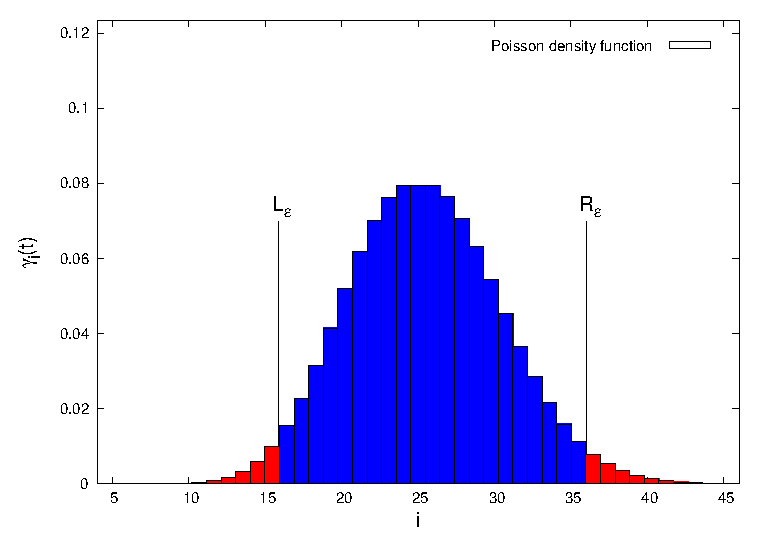
\includegraphics[scale=0.35, angle=0]{poisson.eps}}
			\end{center}
		\end{minipage}
	}
	
	\only<2>{
		\begin{center}
			%see: ../../../../Internal Documents/Steady State Detection/poisson.eps
			\hyperlink{foxglynn<1>}{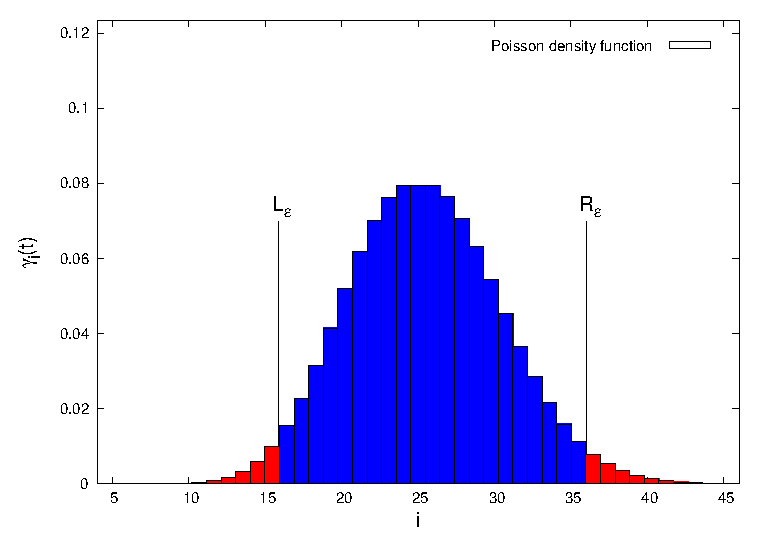
\includegraphics[scale=0.8, angle=0]{poisson.eps}} 
		\end{center}
	}
}

\frame{
	\frametitle{Steady-state, backward computations}
	\begin{alertblock}{Steady-state \cite{ReibmanT_COR88}}
		$\vec{1_{s}} \cdot \mP^{i}$ in (\ref{eq:until_general}) is the power iteration for uniformized DTMC $\mP$ and that is where the steady-state detection comes into play.
	\end{alertblock}
	
	\begin{block}{\alert{Backward computations}}
		Notice that all above is applicable to equation (\ref{eq:fsmc_imr}), see \cite{KatoenKNP_LNCS01}, which gives us
		\begin{equation}
			\vpipt = \sum_{i=0}^{\infty}\pnd \vpi \nonumber
		\end{equation}
		where $ \vpi = \mP^{i} \cdot \vipsi$.
	\end{block}
}

\section{Steady-state detection and $\PspUp{s}{0}{t}$, overview }

\frame{
       \frametitle{Outline}
       \tableofcontents[currentsection]
}

\frame{
	\frametitle{Forward computation, algorithm \cite{MalhotraMT_MR94} }
	\begin{alertblock}{Computations with Steady-state detection}
	\small{
		Let $\exists K \: : \: \nvec{\vpps - \vpsK} \leq \delta$, $\sum_{i=0}^{\ltp} \giqt \leq \frac{\epsilon}{2}$, and $\sum_{i=\rtp}^{\infty} \giqt \leq \frac{\epsilon}{2}$.\\
			\begin{equation}
				\vpipst = \sum_{i=0}^{\infty}\giqt \vpsi \nonumber
			\end{equation}
			\begin{equation}
				\displaystyle
				\vpist = \left\{
				\begin{array}{l}
					\vpsK \text{, if } K < \ltp\\
					\sum_{i=\ltp}^{\rtp}\giqt \vpsi \text{, if } K > \rtp\\
					\sum_{i=\ltp}^{K}\giqt \vpsi + \vpsK \left(1- \sum_{i=0}^{K}\giqt \right) \text{, else}
				\end{array}
				\right .
				\label{eq:ssd_LR}
			\end{equation}
		Then: 
		\begin{equation}
			\alert{ \nvec{\vpipst - \vpist} \leq 2 \delta + \frac{\epsilon}{2}}  \nonumber
		\end{equation}
	}
	\end{alertblock}
}

\frame{
	\frametitle{Criteria}

	\begin{block}{A corollary}
		\begin{equation}
			\nvec{\vpps - \vpsK} \leq \frac{\epsilon}{4} \text{ implies } \nvecinf{\vpipst - \vpist}\leq \epsilon \nonumber
		\end{equation}
	\end{block}
		
	\begin{block}{The actual steady-state detection criteria}
		\begin{itemize}
			\item Take $K = i + M$ if 
				\begin{equation}
					\nvec{{\color[rgb]{0,0,1} \vpsi} - \vpsK} \leq \frac{\epsilon}{4} \nonumber 
				\end{equation}
			\item Check for $K$ every $M$ iterations
		\end{itemize}
	\end{block}
}

\frame{
	\frametitle{The known problems}
	
	\begin{alertblock}{Problems}
		\begin{enumerate}
			\item \emph{The steady-state detection is uncertain} - due to the criteria
			\item \emph{The error bound is not precise} - as derived under an assumption of knowing \emph{real} steady-state. \label{it:p2}
			\item \emph{The norm $\nvec{.}$ is not defined} - was assumed that:
				\begin{equation}
					\nvec{\vpsi} \leq 1 \nonumber
				\end{equation}
			\item \emph{The weights are not considered} - if the complete Fox-Glynn algorithm is used. \label{it:p4}
		\end{enumerate}
	\end{alertblock}
}

\frame{
	\frametitle{Backward computations, algorithm \cite{YounesKNP_TACAS04}}
	\begin{alertblock}{Computations with Steady-state detection}
	\small{
		Let $\exists K \: : \: \nvec{\vpp - \vpK} \leq \delta$, $\sum_{i=0}^{\ltp} \giqt \leq \frac{\epsilon}{2}$, and $\sum_{i=\rtp}^{\infty} \giqt \leq \frac{\epsilon}{2}$.\\
			\begin{equation}
				\vpipt = \sum_{i=0}^{\infty}\giqt \vpi \nonumber
			\end{equation}
			\begin{equation}
				\displaystyle
				\vpit = \left\{
				\begin{array}{l}
					\vpK \text{, if } K < \ltp\\
					\sum_{i=\ltp}^{\rtp}\giqt \vpi \text{, if } K > \rtp\\
					\sum_{i=\ltp}^{K}\giqt \vpi + \vpK \left(1- \sum_{{\color[rgb]{0,0,1}i=\ltp}}^{K}\giqt \right) \text{, else}
				\end{array}
				\right .
				\label{eq:ssd_LR_b}
			\end{equation}
		Then: 
		\begin{equation}
			\alert{ \nvec{\vpipt - \vpit} \leq 2 \delta + \frac{\epsilon}{2}}  \nonumber
		\end{equation}
	}
	\end{alertblock}
}
	
\frame[label=regular]{
	\frametitle{Criteria}

	\begin{block}{A corollary}
		\begin{equation}
			\nvec{\vpp - \vpK} \leq {\color[rgb]{0,0,1} \frac{\epsilon}{8}} \text{ implies } \nvecinf{\vpipt - \vpit}\leq \epsilon \nonumber
		\end{equation}
	\end{block}
		
	\begin{block}{The actual steady-state detection criteria}
		\begin{itemize}
			\item Take $K = i + M$ if 
				\begin{equation}
					\nvec{{\color[rgb]{0,0,1} \vpi} - \vpK} \leq {\color[rgb]{0,0,1} \frac{\epsilon}{8}} \nonumber 
				\end{equation}
			\item Check for $K$ every $M$ iterations
		\end{itemize}
	\end{block}
}

\frame{
	\frametitle{The known problems}
	
	\begin{alertblock}{Problems}
		\begin{enumerate}
			\item \emph{The error bound for (\ref{eq:ssd_LR_b}) can be refined} - $\forall \jinlN{j}{1}{N}, \forall \jinlN{i}{0}{\infty} \: : \: \pij \leq \pilj $. \label{it:p5}
			\item \emph{An additional error is introduced} -  while switching from (\ref{eq:ssd_LR}) to (\ref{eq:ssd_LR_b}), $i=0$ became $i=\ltp$. \label{it:p6}
			\item \emph{The refinement, done in \cite{YounesKNP_TACAS04}, for (\ref{eq:ssd_LR}) and (\ref{eq:ssd_LR_b}) is incorrect} - the length of the error interval does not matter. \label{it:p7} 
		\end{enumerate}
	\end{alertblock}
}

\section{The Fox-Glynn error-bound refinement}

\frame{
       \frametitle{Outline}
       \tableofcontents[currentsection]
}

\frame{
	\frametitle{Choosing the "right" norm}
	\begin{block}{Facts}
		\begin{itemize}
			\item The error estimate, is based on \emph{G}eometrical \emph{C}onvergence
			\item \emph{G.C.} is proved, using \emph{total variation norm} which, in an {$N$-dimensional space}, $\nvecinf{v} = \max_{\jinlN{i}{1}{N}} |v_{i}|$.
			\item In a finite dimensional space all norms are equivalent.
		\end{itemize}
	\end{block}
	
	\begin{alertblock}{Caution!}
		The $\vipsi$ vector is not a distribution, $\forall \jinlN{j}{1}{N}\: : \: 0 \leq \pij \leq 1$.
	\end{alertblock}
	
	\begin{example}
		For $N$ states and Euclidean Norm $\nvece{.}$: \\
		$\:\:\:\:\:\:\:\:\nvece{\sum_{i=0}^{\ltp-1} \giqt \vpi} \nleq \frac{\epsilon}{4}$ {\color[rgb]{1,0,0} BUT}
		$\nvece{\sum_{i=0}^{\ltp-1} \giqt \vpi} \leq \frac{\sqrt{N}}{4}\epsilon$
	\end{example}
}

\frame<1>[label=fgrefined] {
	\frametitle{The Fox-Glynn error-bound refinement}

	\only<1| article:0| trans:0| handout:0>{
		\begin{block}{Errors}
			\begin{itemize}
				\item $\ltp$ and $\rtp$, each, give error $\frac{\epsilon}{4}$
				\item Normalization $\frac{\wi}{W}$gives additional $\frac{\epsilon}{2}$
			\end{itemize}
		\end{block}
	
		\begin{alertblock}{Lemma}
			Let $f$ be a real-valued function with $\|f\| = \sup_{\jinlN{i}{0}{\infty}}|f(i)|$, $f$ does not change sign, and $\sum_{i=\ltp}^{\rtp} \giqt \geq 1 - \frac{\epsilon}{2}$. In exact arithmetic,
			\begin{equation}
				| \sum_{i=0}^{\infty} \giqt f(i) - \frac{1}{W}\sum_{i = \ltp}^{\rtp} \wi f(i)| \leq {\color[rgb]{0,0,1} \frac{\epsilon}{2}} \cdot \|f\|
				\label{pr:fg_imp}
			\end{equation}
		\end{alertblock}

		\vskip1em
		\hyperlink{fgrefined<2>}{\beamergotobutton{Proof details}}
%		\hfill\hyperlinkframestartnext{\beamerskipbutton{Skip proof}}
	}
	\only<2>{% this is only shown in the appendix, where this frame is resumed.
			\begin{proof} 
				Due to the facts that
				{\small
				\begin{eqnarray}
					0 \leq \sum_{i = 0}^{\ltp-1} \giqt +  \sum_{i = \rtp+1}^{\infty} \giqt \leq \frac{\epsilon}{2} \nonumber \\
					- \frac{\epsilon}{2} \leq \sum_{i = \ltp}^{\rtp} (\giqt - \frac{\wi}{W} ) \leq 0 \nonumber \\
					\forall \jinlN{i}{0}{\infty} \: : \: 0 \leq f(i) \leq \|f\| \text{, $f$ is non-negative} \nonumber \\
					\forall \jinlN{i}{0}{\infty} \: : \: -\|f\| \leq f(i) \leq 0 \text{, $f$ is non-positive} \nonumber
				\end{eqnarray}
				}
			\end{proof}
			\only<beamer>{
				\hfill\hyperlink{fgrefined<1>}{\beamerreturnbutton{Return}}
			}
	}
}

\section{Steady-state detection, error-bound refinement}

\frame{
	\frametitle{Refined steady-state detection error}
	\begin{block}{Forward Computations}
	\small{
		Let $\exists K \: : \: \nvecinf{\vpps - \vpsK} \leq \delta$, $\sum_{i=0}^{\ltp} \giqt \leq {\color[rgb]{0,0,1}\frac{\epsilon}{4}}$, $\sum_{i=\rtp}^{\infty} \giqt \leq {\color[rgb]{0,0,1}\frac{\epsilon}{4}}$, and ${\color[rgb]{0,0,1}\Ind} \in 2^{N}$ is a set of indexes.
		\begin{equation}
			\vpipst = \sum_{i=0}^{\infty} \giqt \vpsi \nonumber
		\end{equation}
		\begin{equation}
			%\displaystyle
			\vpist = \left\{
			\begin{array}{l}
				\vpsK \text{, if } K < \ltp \\
				{\color[rgb]{0,0,1}\frac{1}{W}} \sum_{i=\ltp}^{\rtp} {\color[rgb]{0,0,1}\wi} \vpsi \text{, if } K > \rtp\\
				{\color[rgb]{0,0,1}\frac{1}{W}} \sum_{i=\ltp}^{K} {\color[rgb]{0,0,1}\wi} \vpsi + \vpsK \left(1- {\color[rgb]{0,0,1}\frac{1}{W}} \sum_{i={\color[rgb]{0,0,1}\ltp}}^{K}{\color[rgb]{0,0,1}\wi} \right) \text{, else} \\
			\end{array}
			\right .
			\nonumber
		\end{equation}
		Then:
		\begin{equation}
			\alert{ \left| \sum_{j \in \Ind} \left( \pipstj - \pistj \right) \right| \leq 2 \delta {\color[rgb]{0,0,1}|\Ind|} + {\color[rgb]{0,0,1}\frac{3}{4}} \epsilon} \nonumber
		\end{equation}
	}
	\end{block}
}

\frame{
	\frametitle{Refined steady-state detection error}
	\begin{block}{Backward Computations}
	\small{
		Let $\exists K \: : \: \nvecinf{\vpp - \vpK} \leq \delta$, $\sum_{i=0}^{\ltp} \giqt \leq {\color[rgb]{0,0,1}\frac{\epsilon}{4}}$, $\sum_{i=\rtp}^{\infty} \giqt \leq {\color[rgb]{0,0,1}\frac{\epsilon}{4}}$.
		\begin{equation}
			\vpipt = \sum_{i=0}^{\infty} \giqt \vpi \nonumber
		\end{equation}
		\begin{equation}
			%\displaystyle
			\vpit = \left\{
			\begin{array}{l}
				\vpK \text{, if } K < \ltp \\
				{\color[rgb]{0,0,1}\frac{1}{W}} \sum_{i=\ltp}^{\rtp} {\color[rgb]{0,0,1}\wi} \vpi \text{, if } K > \rtp\\
				{\color[rgb]{0,0,1}\frac{1}{W}} \sum_{i=\ltp}^{K} {\color[rgb]{0,0,1}\wi} \vpi + \vpK \left(1- {\color[rgb]{0,0,1}\frac{1}{W}} \sum_{i={\color[rgb]{0,0,1}\ltp}}^{K}{\color[rgb]{0,0,1}\wi} \right) \text{, else} \\
			\end{array}
			\right .
			\nonumber
		\end{equation}
		Then:
		\begin{equation}
			\alert{ \nvecinf{ \vpipt - \vpit } \leq {\color[rgb]{0,0,1}\delta} + {\color[rgb]{0,0,1}\frac{3}{4}} \epsilon }\nonumber
		\end{equation}
	}
	\end{block}
}

\frame<1>[label=frdcomput]{
	\frametitle{Steadt-state detection criteria}
	\only<1>{
		\begin{alertblock}{Forward computations Criterion}
			\begin{enumerate}
				\item Steady-state is detected if $\nvecinf{{\color[rgb]{0,0,1}\vpps} - \vpsK} \leq \frac{\epsilon}{8 |\SPsi|}$
				\item Use the Fox-Glynn algorithm with desired error $\frac{\epsilon}{2}$
				\item Then the overall error bound for the computed probability $\PspUp{s}{0}{t}$ will be $\epsilon$
			\end{enumerate}
		\end{alertblock}
		\hyperlink{frdcomput<2>}{\beamergotobutton{Error bound details}}

		\begin{alertblock}{Backward computations Criterion}
			\begin{enumerate}
				\item Steady-state is detected if $\nvecinf{{\color[rgb]{0,0,1}\vpp} - \vpK} \leq \frac{\epsilon}{4}$
				\item Use the Fox-Glynn algorithm with desired error $\frac{\epsilon}{2}$
				\item Then $\forall \jinlN{j}{1}{N}$ the overall error bound for computed probability $\PspUp{j}{0}{t}$, will be $\epsilon$
			\end{enumerate}
		\end{alertblock}
		\hyperlink{frdcomput<3>}{\beamergotobutton{Error bound details}}
	}
	
	\only<2>{
		\begin{block}{Forward computations Details}
			{\small Assuming $\forall i \geq K \: : \: \nvecinf{\vpps - \vpsi} \leq \delta$ and the Fox-Glynn algorithm's error bound $\frac{\epsilon}{2}$ we have:}
			{\tiny
			\begin{enumerate}
				\item ($K > \rtp$): 
					\begin{equation}
						- \frac{\epsilon}{2} \leq \sum_{j \in \SPsi}\left(\pipstj - \pistj\right) \leq \frac{\epsilon}{2} \nonumber
					\end{equation}
				\item ($\ltp \leq K \leq \rtp$):
					\begin{equation}           
						-  2\delta |\SPsi| - \frac{3}{4}\epsilon \leq \sum_{j \in \SPsi} \left( \pipstj - \pistj \right) \leq  2 \delta |\SPsi| + \frac{3}{4} \epsilon \nonumber
					\end{equation}
				\item ($K < \ltp$): 
					\begin{equation}           
						-  2\delta |\SPsi| - \frac{1}{4}\epsilon \leq \sum_{j \in \SPsi} \left( \pipstj - \pistj \right) \leq  2 \delta |\SPsi| + \frac{1}{4} \epsilon \nonumber
					\end{equation}
			\end{enumerate}
			}
		\end{block}
		\only<beamer>{
			\hfill\hyperlink{frdcomput<1>}{\beamerreturnbutton{Return}}
		}
	}
	
	\only<3>{
		\begin{block}{Backward computations Details}
			{\small Assuming $\forall i \geq K \: : \: \nvecinf{\vpp - \vpi} \leq \delta$ and the Fox-Glynn algorithm's error bound $\frac{\epsilon}{2}$ we have:}
			{\tiny
			\begin{enumerate}
				\item ($K > \rtp$): 
					\begin{equation}
						- \frac{\epsilon}{2} \leq \piptj - \pitj \leq \frac{\epsilon}{2} \nonumber
					\end{equation}
				\item ($\ltp \leq K \leq \rtp$):
					\begin{equation}           
						-  \delta - \frac{3}{4} \epsilon \leq \piptj - \pitj \leq  \delta + \frac{3}{4} \epsilon \nonumber
					\end{equation}
				\item ($K < \ltp$): 
					\begin{equation}           
						-  \delta - \frac{1}{4}\epsilon \leq \piptj - \pitj \leq  \delta + \frac{1}{4} \epsilon \nonumber
					\end{equation}
			\end{enumerate}
			}
		\end{block}
		\only<beamer>{
			\hfill\hyperlink{frdcomput<1>}{\beamerreturnbutton{Return}}
		}
	}
}

\section{Improved steady-state detection}

\frame{
       \frametitle{Outline}
       \tableofcontents[currentsection]
}

\frame<1>[label=absorb1]{
	\frametitle{Making states absorbing I}
	\only<1>{
		\begin{definition}
			For a directed graph a subgraph is a \emph{Bottom Strongly Connected Component} (BSCC) if it is a maximum strongly connected component such that it has no edges to outside its vertices.
		\end{definition}
		\begin{alertblock}{Lemma}
			If $\mQnpvp$ has a BSCC containing at least one $\Phi$ state then all its states are $\Phi$ states.
			\label{pr:bscc_phi}
		\end{alertblock}
		\hyperlink{absorb1<2>}{\beamergotobutton{Proof details}}
		\begin{block}{Where}
			$\mQ$ is a generator matrix, $\Phi$ and $\Psi$ are CSL state formulas
		\end{block}
	}
	\only<2>{
		\begin{proof}
			The case of a single state BSCC is trivial.
			
			The rest is also trivial, by contradiction.
			
			Let $B$ be a BSCC of $\mQ [ \npvp ]$ such that it has at least two states, $s_{\Phi} \in \SPhi$, $s_{\neg \Phi} \in \Sat{\neg \Phi}$ and $s_{\Phi}, \: s_{\neg \Phi} \in B$. All $\neg \Phi$ states in $\mQ [ \npvp ]$ are made absorbing, thus the $s_{\neg \Phi}$ state has only one self-loop transition. This yields that $s_{\neg \Phi} \not \in B$. 
			
			Contradiction.
		\end{proof}
		\only<beamer>{
			\hfill\hyperlink{absorb1<1>}{\beamerreturnbutton{Return}}
		}
	}
}

\frame<1>[label=absorb2]{
	\frametitle{Making states absorbing II}
	\only<1>{
		\begin{definition}
			Define
			 {\tiny $B_{ \Phi, \Psi }  = \left\{ s \in B \cap \left( \SPhi \setminus \SPsi \right) | B \: is \: a \: BSCC \: in \: \mQ \left[ \npvp \right] \right\}$ }

			Define $\mQ^{B}[\npvp]$ obtained from $\mQ [ \npvp ]$ by making all $B_{ \Phi, \Psi }$ states absorbing.
		\end{definition}
		\begin{definition}
			Let $\PZsf{\mQ}{s}{\Phi}$ be the probability $\Psf{s}{\Phi}$ of satisfying CSL state formula $\Phi$ in state $s$, for the CTMC, defined by the generator matrix $\mQ$.
		\end{definition}
		\begin{alertblock}{Theorem}
			{\small $ \PZspUp{\mQ}{s}{0}{t} = \PZsttUp{\mQnpvp}{s}{t}{t} = \PZsttUp{\mQ^{B}[\npvp]}{s}{t}{t}$ }
		\end{alertblock}
		\hyperlink{absorb2<2>}{\beamergotobutton{Proof details}}
	}
	
	\only<2>{
		\begin{proof}
		The first part $\PZspUp{\mQ}{s}{0}{t} = \PZsttUp{\mQnpvp}{s}{t}{t}$ was proved in \cite{BaierHHK_TSE03}.
		
		The second part $\PZsttUp{\mQnpvp}{s}{t}{t} = \PZsttUp{\mQ^{B}[\npvp]}{s}{t}{t}$ is valid due to the fact, that if there is a BSCC consisting of $\SPhi$ states then $\SPsi$ states are not reachable from it.
		
		Unless it is a trivial case when a BSCC consists of one state $s$ which satisfies both $\Phi$ and $\Psi$ formulas, but in this case it is already made absorbing while obtaining $\mQ[\npvp]$.
		\end{proof}
		\only<beamer>{
			\hfill\hyperlink{absorb2<1>}{\beamerreturnbutton{Return}}
		}
	}
 }

\frame{
	\frametitle{Precise steady-state detection, Forward computations}
	\begin{alertblock}{Theorem}
		For a uniformized CTMC $\mP_{B}$, obtained from the generator matrix $\mQBnpvp$:
		{\small \begin{equation}
			\forall \delta \geq 0 \: : \: \sum_{j \in \SPhi \setminus \left( \BPsi \cup \SPsi \right)} \psij \leq \delta \Rightarrow \nvecinf{\vpps - \vpsi} \leq \delta \nonumber
		\end{equation}}
		 \label{th:criteria_1}
	\end{alertblock}
	
	\begin{block}{Where}
		\begin{description}
			\item[$\vpps$] - the steady-state of $\mP_{B}$ when starting from $s$
			\item[$\psij$] - the $j$'th component of $\vpsi = \vec{1_{s}} \cdot \mP_{B}^{i} $
		\end{description}
	\end{block}
}

\frame[label= precise]{
	\frametitle{Precise steady-state detection, Backward computations}
	\begin{alertblock}{Theorem}
		For a uniformized CTMC $\mP_{B}$, obtained from the generator matrix $\mQBnpvp$:
		{\small \begin{equation}
			\forall \delta \geq 0 \: : \: \nvecinf{ \vec{1} - \left( \vpi + \vbpi \right) } \leq \delta \Rightarrow \nvecinf{\vpp - \vpi} \leq \delta \nonumber
		\end{equation}}
		\label{th:criteria_2}
	\end{alertblock}
	\begin{block}{Where}
		\begin{minipage}{0.5\linewidth}
			\begin{description}
				\item[$\vbpi$] = $\mP_{B}^{i} \cdot \vibad$
				\item[$\vpp$] = $\lim_{i \rightarrow \infty} \mP_{B}^{i} \cdot \vipsi$
			\end{description}
		\end{minipage} \hfill
		\begin{minipage}{0.48\linewidth}
			\begin{description}
				\item[$\vpi$] = $\mP_{B}^{i} \cdot \vipsi$
			\end{description}
		\end{minipage}
	\end{block}
}

\section{Experiments}

\frame{
       \frametitle{Outline}
       \tableofcontents[currentsection]
}

\frame{
	\frametitle{Premature steady-state detection \cite{MassinkKL_DSN04}}
	{\small
	\begin{block}{Tools}
		\begin{center}
			\begin{tabular}{|c|r|r|}
				\hline
					Tool Name & Reference & S.s.d. method \\
				\hline
					\prism & \cite{KwiatkowskaNP_QEST04} & \hyperlink{regular}{\emph{regular}}\\
				\hline
					\etmcc & \cite{HermansKMS_IJSTTT03} & \hyperlink{regular}{\emph{regular}}\\
				\hline
					\mrmc & \cite{KatoenKZ_QEST05} & \hyperlink{precise}{\emph{precise}}\\
				\hline
			\end{tabular}
		\end{center}
	\end{block}
	}
	
	\begin{example}
	{\tiny
		\begin{figure}
			\begin{center}
				\begin{picture}(80,25)(0,0)
					\def\x1{10}\def\y1{10}
					\node(n1)(\x1,\y1){$1$}
					\def\x2{40}\def\y2{10}
					\node(n2)(\x2,\y2){$0$}      
					\def\x3{70}\def\y3{10}
					\node(n3)(\x3,\y3){$2$}
      
					\gasset{ExtNL=y, NLdist=1, ilength=-2}
					\nodelabel[NLangle=270](n1){$\Phi$}
					\nodelabel[NLangle=270](n2){$\Phi$}
					\nodelabel[NLangle=270](n3){$\Psi$}
    
					\drawedge[curvedepth=8](n2,n1){$0.9999$}
					\drawedge[curvedepth=8](n1,n2){$0.00005$}
					\drawedge(n2,n3){$0.00005$}
				\end{picture}
			\end{center}
			\caption{A slowly convergent CTMC \label{gr:sc_mc}}
		\end{figure}
	}
	\end{example}
}

\frame<1>[label=rslt]{
	\frametitle{Computational results}

	\only<1>{
		\begin{example}
			{\tiny
			\begin{center}
				\begin{tabular}{|l|c|c|c|c|}								\hline
					Tool 		& Error &  $K$  & $\mP^{K} \cdot \vipsi$ & $\vpp$  \\
					\hline
					\prism (abs)	& $10^{-6}$ &	 2 & ($5.00025 \cdot 10^{-5}$, $2.5 \cdot 10^{-9}$, 1.0) & \multirow{4}{*}{(1.0, 1.0, 1.0)} \\
					\prism (rel)	& $10^{-1}$ &	12 & ($5.00275 \cdot 10^{-5}$, $2.75 \cdot 10^{-8}$, 1.0) & \\
					\etmcc		& $10^{-6}$ &	20 & ($5.00475 \cdot 10^{-5}$, $4.75 \cdot 10^{-8}$, 1.0) & \\
					\mrmc		& $10^{-6}$ & ---	& --- & \\
					\hline
				\end{tabular}
			\end{center}
			}
		\end{example}
		\begin{minipage}{0.48\linewidth}
			\begin{center}
				\hyperlink{rslt<2>}{\includegraphics[scale=0.45, angle=0]{../../../../../experiments/26_08_2005/CSL/ssd_02/results.eps}}
			\end{center}
		\end{minipage} \hfill
		\begin{minipage}{0.48\linewidth}
			\begin{center}
				\hyperlink{rslt<3>}{\includegraphics[scale=0.45, angle=0]{../../../../../experiments/26_08_2005/CSL/ssd_02/results_ext.eps}}
			\end{center}
		\end{minipage}
	}

	\only<2>{
		\begin{figure}
			\begin{center}
				\hyperlink{rslt<1>}{\includegraphics[scale=0.8, angle=0]{../../../../../experiments/26_08_2005/CSL/ssd_02/results.eps}}
			\end{center}
			\caption{Results for formula $\PspUp{0}{0}{t}$ \label{gr:prob_2}}
		\end{figure}
	}
	
	\only<3>{
		\begin{figure}
			\begin{center}
				\hyperlink{rslt<1>}{\includegraphics[scale=0.8, angle=0]{../../../../../experiments/26_08_2005/CSL/ssd_02/results_ext.eps}}
			\end{center}
			\caption{Results for formula $\PspUp{0}{0}{t}$, extended time interval \label{gr:prob_2}}
		\end{figure}
	}
}

\frame{
	\frametitle{Workstation cluster \cite{HaverkortHK_SRDS00}}

	\begin{figure}[h!]
		\begin{center}
			\includegraphics[scale=0.8, angle=0]{../../../../../experiments/24_10_2005/CSL/ssd_03/results.eps}
		\end{center}
	\caption{Time required to compute $\Psf{4167}{\ppUp{true}{0}{t}{!minimum}}$ probabilities}
	\end{figure}
}

\frame{
	\frametitle{Computation time}

	\begin{figure}[h!]
		\begin{center}
			\includegraphics[scale=0.8, angle=0]{../../../../../experiments/30_08_2005/CSL/ssd_03/csl_bounded_until_10/results_time.eps}
		\end{center}
	\caption{Time required to compute $\PspUp{0}{0}{t}$ probabilities}
	\end{figure}
}

\section{Related works}

\frame{
       \frametitle{Outline}
       \tableofcontents[currentsection]
}

\frame{
       \frametitle{Related, ...}
       \begin{block}{..., but unused}
       	\begin{description}
			\item[\cite{Sericola_TC99}] - the method, based on Uniformization, to determine the \emph{point availability} and \emph{expected interval availability} of a repairable computer system modeled as a Markov chain with steady-state detection. \\
				\emph{\alert{Limitation:} Results are only applicable for irreducible Markov Chains}
			\item[\cite{Neuts_81}] - \emph{Phase Type} distribution, has a  theorem limiting the time before absorption.\\
				\emph{\alert{Limitation:} Transient states must form an irreducible matrix}
		\end{description}
       \end{block}
}

\section{Conclusions}

\frame{
       \frametitle{Outline}
       \tableofcontents[currentsection]
}

\frame{
       \frametitle{Conclusions}
	\begin{exampleblock}{Results}
		\begin{enumerate}
			\item The error bound corrections
				\begin{itemize}
					\item Steady-state detection - fixed multiple problems
					\item The Fox-Glynn algorithm - partial error-bound refinement 
					\item Uniformization using the Fox-Glynn - added weights influence
				\end{itemize}
			\item Precise steady-state detection criteria
				\begin{itemize}
					\item Forward computations - preserves time complexity,\\
							computation time may slightly increase
					\item Backward computations - preserves time complexity,\\
							computation time may approximately double
				\end{itemize}			
		\end{enumerate}
	\end{exampleblock}
}

%BIBLIOGRAPHY
\section{Literature}

\frame{
       \frametitle{Outline}
       \tableofcontents[currentsection]
}

{\tiny \bibliography{../../../../BibTex/global_etmcc}}

%APPENDIX
\appendix

\AtBeginSubsection{}

\section{\appendixname}

\frame{\frametitle{Appendix Outline}\tableofcontents}

\subsection{Numerical computation of  $\PspUp{s}{0}{t}$}

\againframe<beamer| beamer:2>{foxglynn}

\subsection{The Fox-Glynn, steady-state detection, error bound}

\againframe<beamer| beamer:2>{fgrefined}

\againframe<beamer| beamer:2>{frdcomput}

\againframe<beamer| beamer:3>{frdcomput}

\subsection{Improved steady-state detection}

\againframe<beamer| beamer:2>{absorb1}

\againframe<beamer| beamer:2>{absorb2}

\subsection{An example}

\againframe<beamer| beamer:2>{rslt}

\againframe<beamer| beamer:3>{rslt}

\end{document}
